\section{Running Example: Simple Calculation FB}
\label{sec::running_example}
As a running example, we use an FB that performs a simple calculation (Figure~\ref{fig:running_example}) based on the inputs according to the formula \texttt{DO1:=DI1+2*DI2}. It contains the following language elements:

\begin{figure}[b]
    \centering
    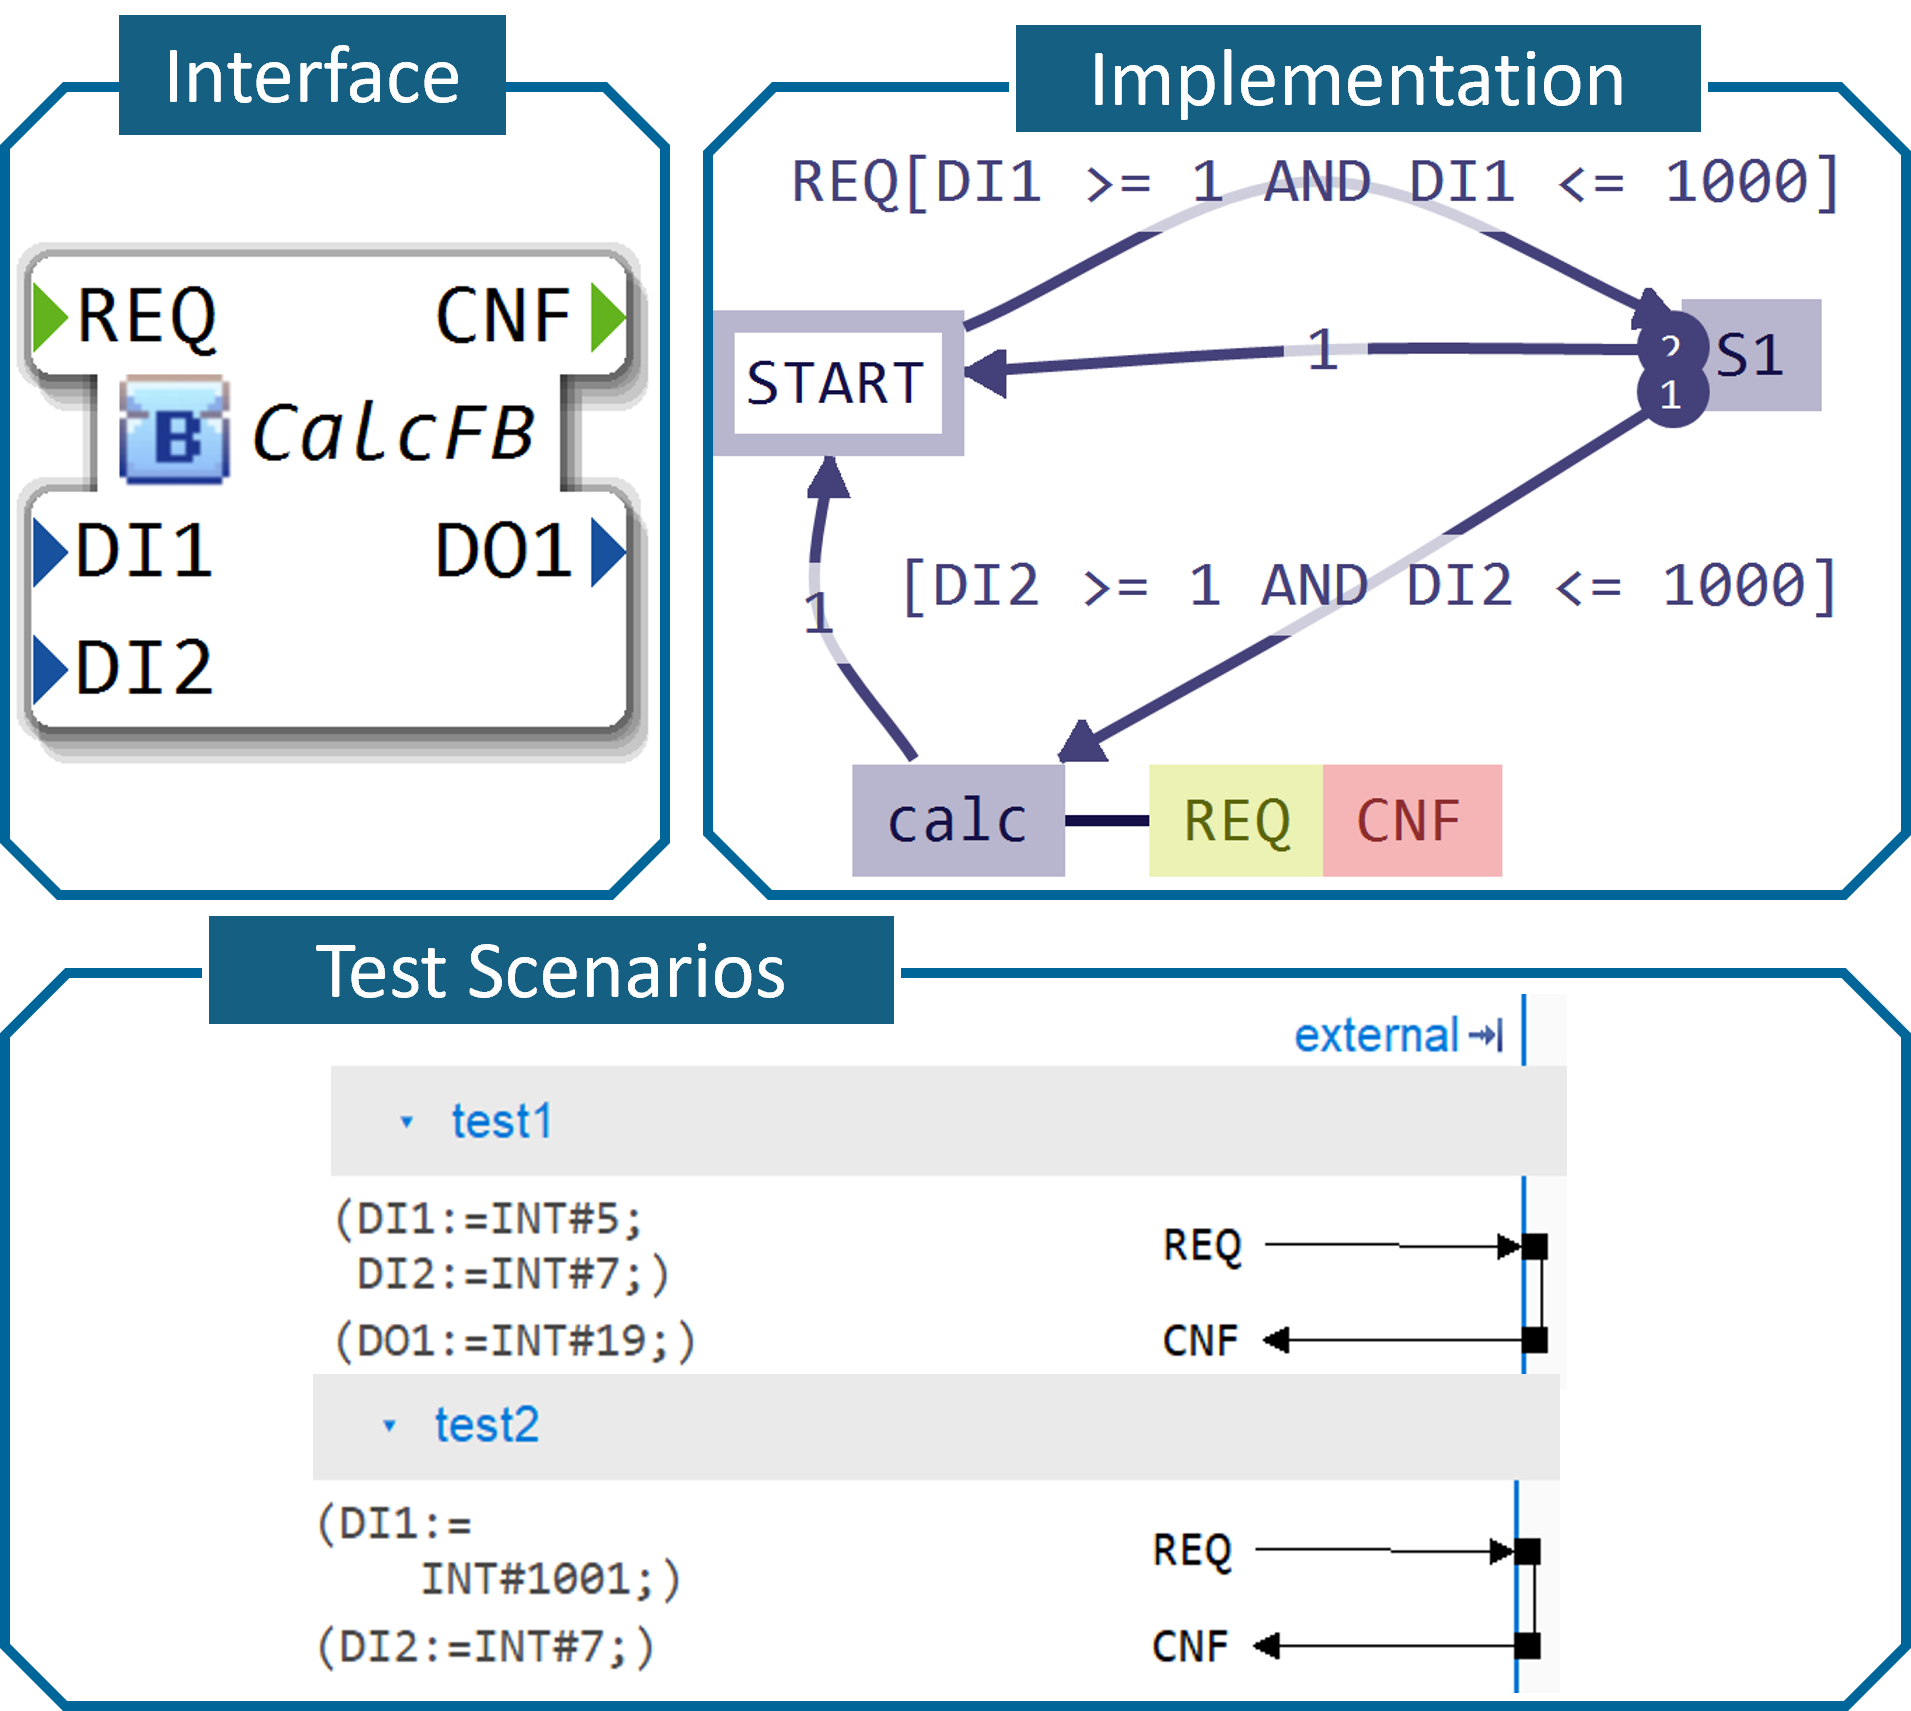
\includegraphics[width=0.75\columnwidth]{OJIES_2024/Figures/RunningExample.png}
    \caption{Running Example: FB performing simple calculation. FB interface defining the component, implementation as state diagram, and two usage scenarios modelled as service sequences.}
    \label{fig:running_example}
\end{figure}
\begin{figure*}[t!]
	\centering
	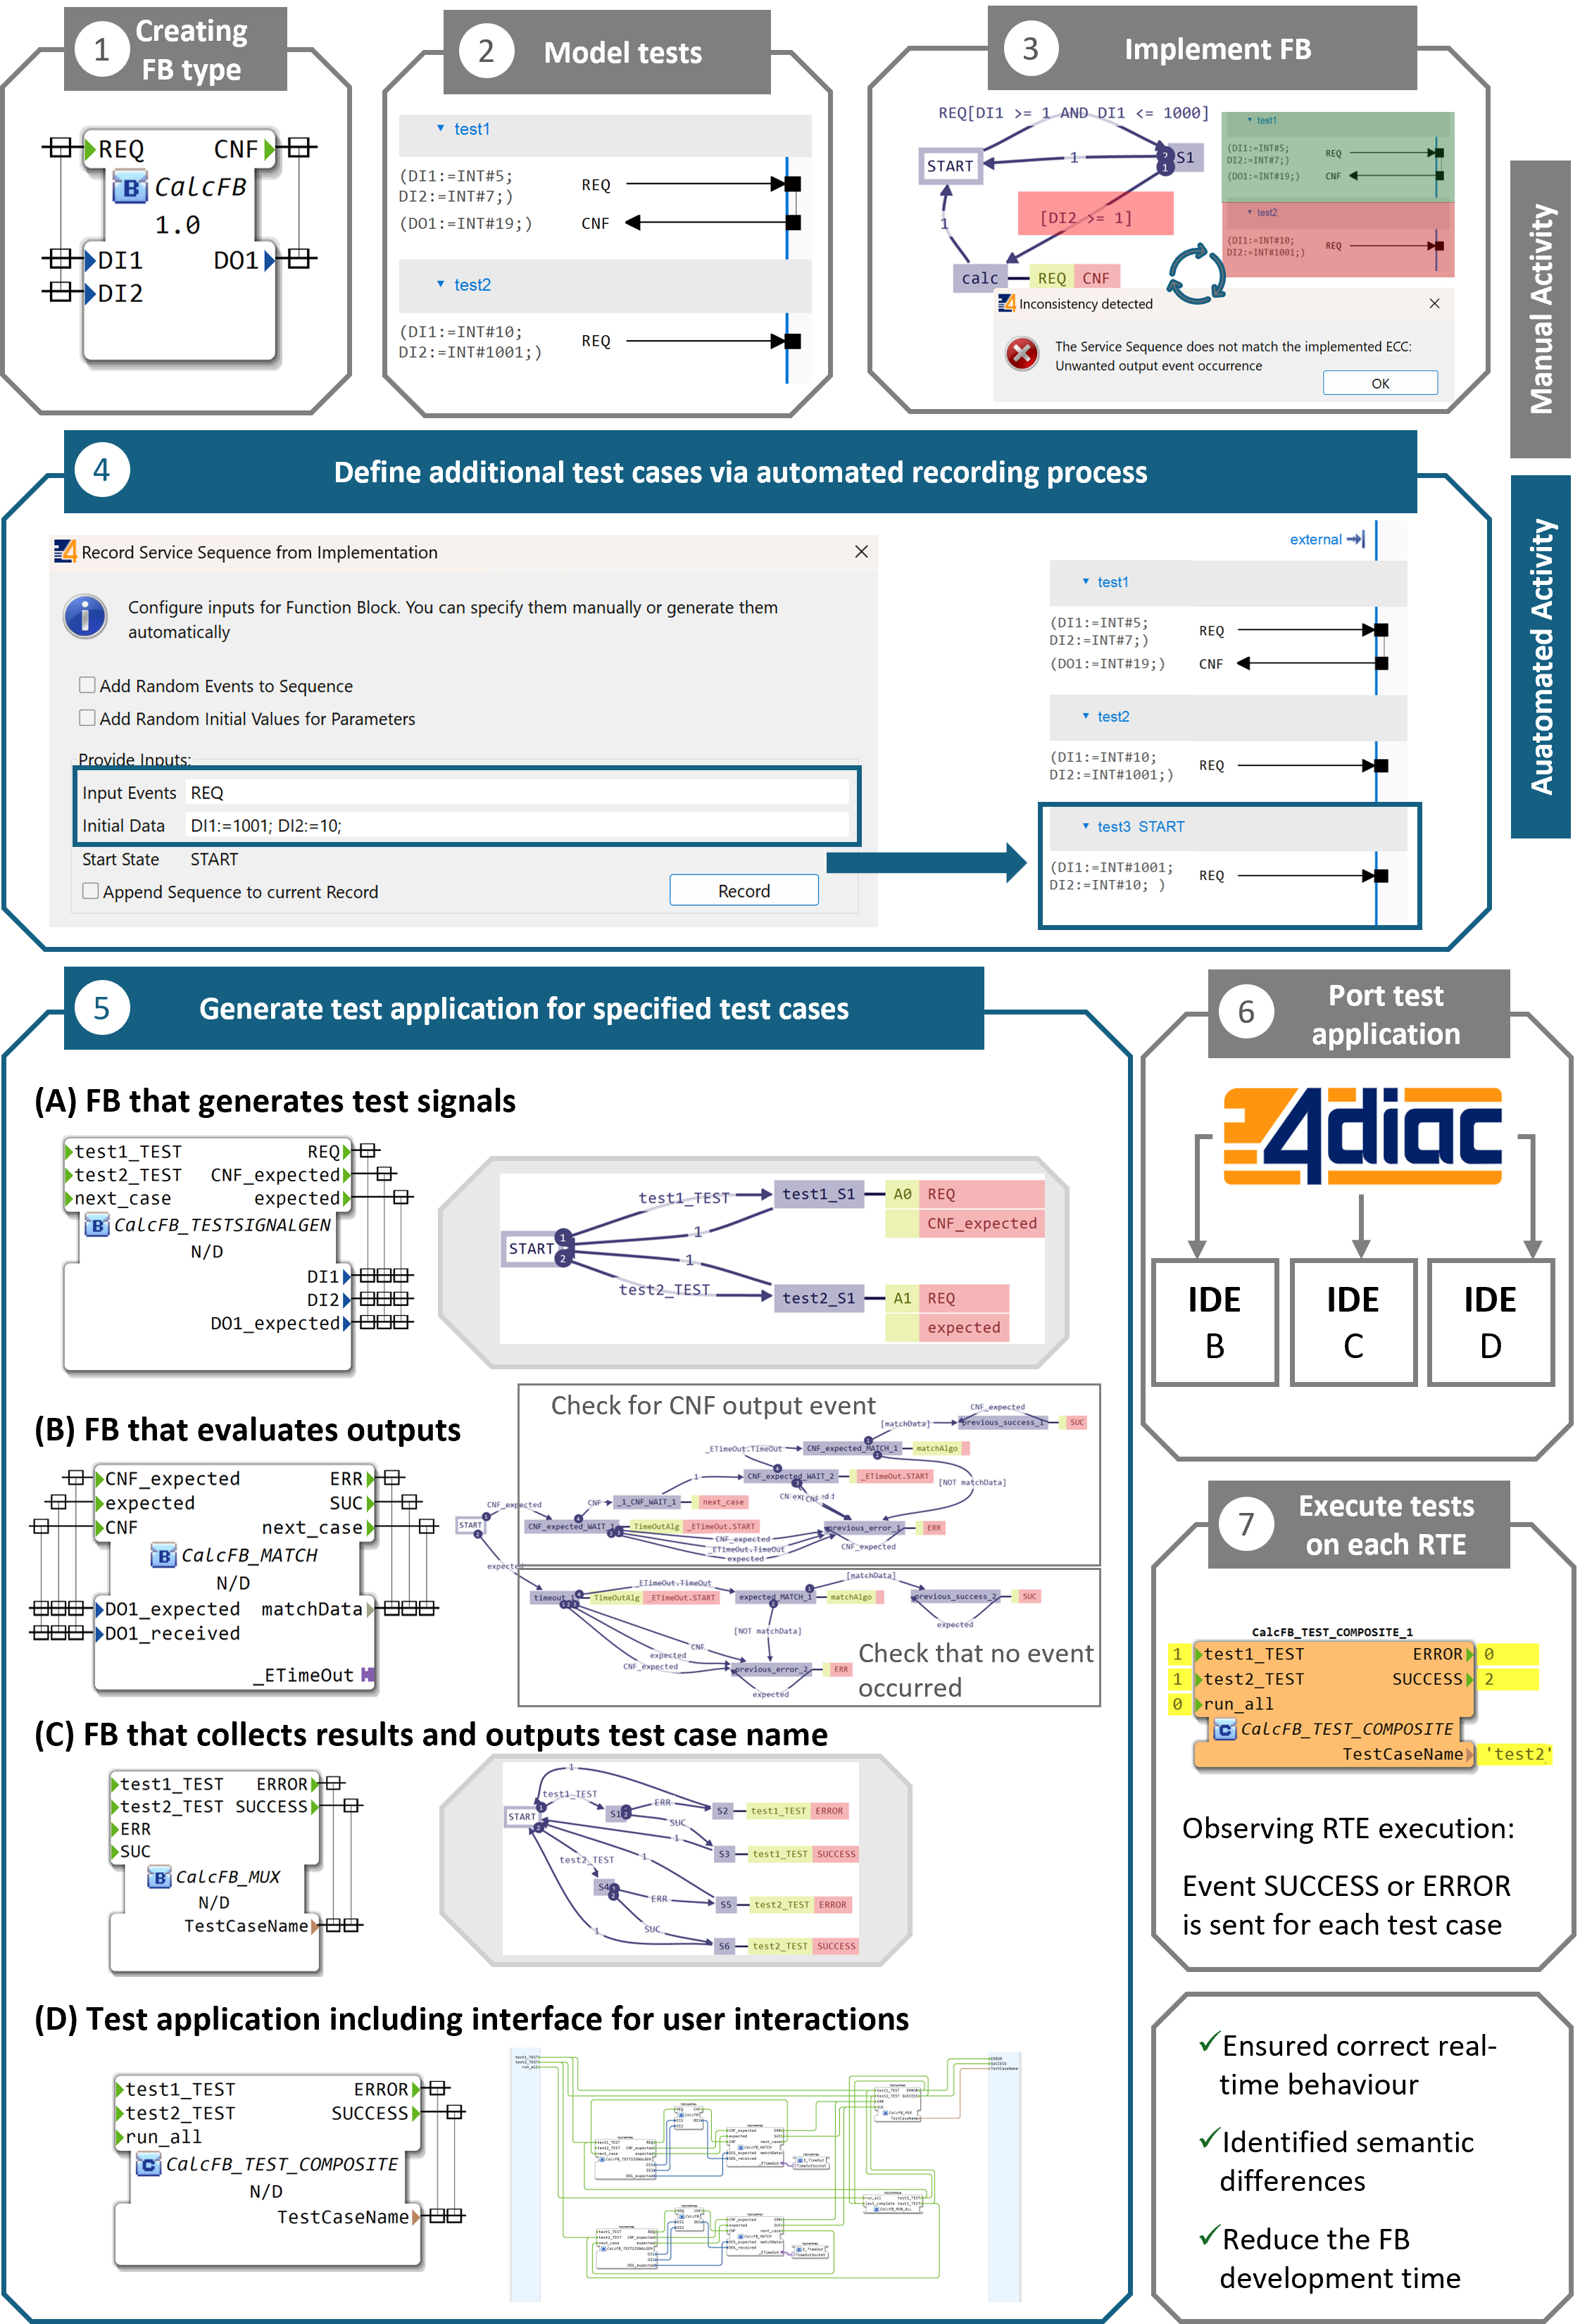
\includegraphics[width=0.85\textwidth]{OJIES_2024/Figures/methodology_complete.png}
	\caption{Overview of process for testing FBs across various software platforms. The seven-step process is partly automated with tools (blue boxes), partly it requires tool-assisted manual development. The test application can be ported to tools of various vendors and validate the expected behaviour of an FB directly in the target RTE, thus, possibly identifying differences in the execution semantics that affect the FB under test.}
	\label{fig::methodology}
\end{figure*}

\begin{itemize}
   \item Input event \texttt{REQ} triggers the calculation.
   \item Data inputs \texttt{DI1}, \texttt{DI2} receive values from other FBs and are used in the algorithm.
   \item The data output \texttt{DO1} stores the result of the algorithm.
   \item The output event \texttt{CNF} is issued to indicate that the algorithm was completed and that the output result is ready to be used by other FBs.
   \item The algorithm \texttt{REQ} within the FB is executed whenever the input event \texttt{REQ} occurs. The algorithm assigns the result of the formula to the output variable DO1.
%Once the algorithm execution is completed, the function block triggers the CNF event to indicate that the output result is ready to be used or transmitted to other function blocks.
\end{itemize}

In our example, the FB performs the calculation if the values of \texttt{DI1} and \texttt{DI2} are between 1 and 1000 (cf. implementation of the state diagram in Figure~\ref{fig:running_example}). When triggering the \texttt{REQ} event with appropriate input values, the FB executes the algorithm and produces the respective output. Both cases are modelled as service sequences and serve as test scenarios for the running example.
%\subsection{Running Example: Service Model}

